%% For double-blind review submission, w/o CCS and ACM Reference (max submission space)
\documentclass[acmsmall,review,anonymous]{acmart}\settopmatter{printfolios=true,printccs=false,printacmref=false}
%% For double-blind review submission, w/ CCS and ACM Reference
%\documentclass[acmsmall,review,anonymous]{acmart}\settopmatter{printfolios=true}
%% For single-blind review submission, w/o CCS and ACM Reference (max submission space)
%\documentclass[acmsmall,review]{acmart}\settopmatter{printfolios=true,printccs=false,printacmref=false}
%% For single-blind review submission, w/ CCS and ACM Reference
%\documentclass[acmsmall,review]{acmart}\settopmatter{printfolios=true}
%% For final camera-ready submission, w/ required CCS and ACM Reference
%\documentclass[acmsmall]{acmart}\settopmatter{}


%% Journal information
%% Supplied to authors by publisher for camera-ready submission;
%% use defaults for review submission.
\acmJournal{PACMPL}
\acmVolume{1}
\acmNumber{CONF} % CONF = POPL or ICFP or OOPSLA
\acmArticle{1}
\acmYear{2018}
\acmMonth{1}
\acmDOI{} % \acmDOI{10.1145/nnnnnnn.nnnnnnn}
\startPage{1}

%% Copyright information
%% Supplied to authors (based on authors' rights management selection;
%% see authors.acm.org) by publisher for camera-ready submission;
%% use 'none' for review submission.
\setcopyright{none}
%\setcopyright{acmcopyright}
%\setcopyright{acmlicensed}
%\setcopyright{rightsretained}
%\copyrightyear{2018}           %% If different from \acmYear

%% Bibliography style
\bibliographystyle{ACM-Reference-Format}
%% Citation style
%% Note: author/year citations are required for papers published as an
%% issue of PACMPL.
\citestyle{acmauthoryear}   %% For author/year citations


%%%%%%%%%%%%%%%%%%%%%%%%%%%%%%%%%%%%%%%%%%%%%%%%%%%%%%%%%%%%%%%%%%%%%%
%% Note: Authors migrating a paper from PACMPL format to traditional
%% SIGPLAN proceedings format must update the '\documentclass' and
%% topmatter commands above; see 'acmart-sigplanproc-template.tex'.
%%%%%%%%%%%%%%%%%%%%%%%%%%%%%%%%%%%%%%%%%%%%%%%%%%%%%%%%%%%%%%%%%%%%%%


%% Some recommended packages.
\usepackage{booktabs}   %% For formal tables:
                        %% http://ctan.org/pkg/booktabs
\usepackage{subcaption} %% For complex figures with subfigures/subcaptions
                        %% http://ctan.org/pkg/subcaption
\usepackage{catchfilebetweentags} %% For importing code snippets
\usepackage{lineno} %% For line numbers on code snippets
\usepackage{pgfplots}
\usepackage{multicol}
\usepackage{fancyvrb}
\usepackage{wrapfig}

%%%%%%%%%%%%%%%%%%%%%%%%%%%%%%%%%%%%%%%%%%%%%%%%%%%%%%%%%%%%%%%%%%%%%%%%%%%%%%%%
%% Agda special Characters
%%%%%%%%%%%%%%%%%%%%%%%%%%%%%%%%%%%%%%%%%%%%%%%%%%%%%%%%%%%%%%%%%%%%%%%%%%%%%%%%
\usepackage{amssymb}
\usepackage{turnstile}
\usepackage{bbm}
\usepackage[greek, english]{babel}
\usepackage{MnSymbol}
\usepackage{stmaryrd}
\usepackage{csquotes}
\newcommand\doubleplus{+\kern-1.3ex+\kern0.8ex}
\newcommand\mdoubleplus{\ensuremath{\mathbin{+\mkern-8mu+}}}
\makeatletter
\newcommand\incircbin
{%
  \mathpalette\@incircbin
}
\newcommand\@incircbin[2]
{%
  \mathbin%
  {%
    \ooalign{\hidewidth$#1#2$\hidewidth\crcr$#1\bigcirc$}%
  }%
}
\newcommand{\oeq}{\ensuremath{\incircbin{=}}}
\makeatother
\makeatletter
\newcommand\insquarebin
{%
  \mathpalette\@insquarebin
}
\newcommand\@insquarebin[2]
{%
  \mathbin%
  {%
    \ooalign{\hidewidth$#1#2$\hidewidth\crcr$#1\bigbox$}%
  }%
}
\newcommand{\sqtri}{\ensuremath{\insquarebin{\triangle}}}
\makeatother
\usepackage{ucs}
\DeclareUnicodeCharacter{8759}{\ensuremath{\squaredots}}
\DeclareUnicodeCharacter{951}{\textgreek{\texteta}}
\DeclareUnicodeCharacter{737}{\ensuremath{^\text{l}}}
\DeclareUnicodeCharacter{691}{\ensuremath{^\text{r}}}
\DeclareUnicodeCharacter{7523}{\ensuremath{_\text{r}}}
\DeclareUnicodeCharacter{8718}{\ensuremath{\blacksquare}}
\DeclareUnicodeCharacter{957}{\textgreek{\textnu}}
\DeclareUnicodeCharacter{961}{\textgreek{\textrho}}
\DeclareUnicodeCharacter{929}{\textgreek{\textRho}}
\DeclareUnicodeCharacter{954}{\textgreek{\textkappa}}
\DeclareUnicodeCharacter{10214}{\ensuremath{\lsem}}
\DeclareUnicodeCharacter{10215}{\ensuremath{\rsem}}
\DeclareUnicodeCharacter{8857}{\mdoubleplus}
\DeclareUnicodeCharacter{8860}{\oeq}
\DeclareUnicodeCharacter{9043}{\ensuremath{\sqtri}}
\DeclareUnicodeCharacter{928}{\textgreek{\textPi}}
\DeclareUnicodeCharacter{922}{\textgreek{\textKappa}}
\DeclareUnicodeCharacter{931}{\textgreek{\textSigma}}
\DeclareUnicodeCharacter{916}{\textgreek{\textDelta}}
\DeclareUnicodeCharacter{921}{\textgreek{\textIota}}
\DeclareUnicodeCharacter{8779}{\ensuremath{\backtriplesim}}
\DeclareUnicodeCharacter{8799}{\ensuremath{\stackrel{?}{=}}}
\DeclareUnicodeCharacter{10181}{\ensuremath{\lbag}}
\DeclareUnicodeCharacter{10182}{\ensuremath{\rbag}}
\DeclareUnicodeCharacter{8760}{\ensuremath{-}}
\usepackage[references]{agda}

\newcommand{\Nat}{\AgdaDatatype{ℕ}}
%%%%%%%%%%%%%%%%%%%%%%%%%%%%%%%%%%%%%%%%%%%%%%%%%%%%%%%%%%%%%%%%%%%%%%%%%%%%%%%%


\begin{document}

%% Title information
\title[Reading and Writing Arithmetic]{Reading and Writing Arithmetic: Automating Ring Equalities
  in Agda}

%% Author information
%% Contents and number of authors suppressed with 'anonymous'.
%% Each author should be introduced by \author, followed by
%% \authornote (optional), \orcid (optional), \affiliation, and
%% \email.
%% An author may have multiple affiliations and/or emails; repeat the
%% appropriate command.
%% Many elements are not rendered, but should be provided for metadata
%% extraction tools.

%% Author with single affiliation.
\author{Donnacha Oisín Kidney}
\authornote{with author1 note}          %% \authornote is optional;
                                        %% can be repeated if necessary
\orcid{nnnn-nnnn-nnnn-nnnn}             %% \orcid is optional
\affiliation{
  \position{Position1}
  \department{Department1}              %% \department is recommended
  \institution{Institution1}            %% \institution is required
  \streetaddress{Street1 Address1}
  \city{City1}
  \state{State1}
  \postcode{Post-Code1}
  \country{Country1}                    %% \country is recommended
}
\email{first1.last1@inst1.edu}          %% \email is recommended

%% Author with two affiliations and emails.
\author{First2 Last2}
\authornote{with author2 note}          %% \authornote is optional;
                                        %% can be repeated if necessary
\orcid{nnnn-nnnn-nnnn-nnnn}             %% \orcid is optional
\affiliation{
  \position{Position2a}
  \department{Department2a}             %% \department is recommended
  \institution{Institution2a}           %% \institution is required
  \streetaddress{Street2a Address2a}
  \city{City2a}
  \state{State2a}
  \postcode{Post-Code2a}
  \country{Country2a}                   %% \country is recommended
}
\email{first2.last2@inst2a.com}         %% \email is recommended
\affiliation{
  \position{Position2b}
  \department{Department2b}             %% \department is recommended
  \institution{Institution2b}           %% \institution is required
  \streetaddress{Street3b Address2b}
  \city{City2b}
  \state{State2b}
  \postcode{Post-Code2b}
  \country{Country2b}                   %% \country is recommended
}
\email{first2.last2@inst2b.org}         %% \email is recommended



%% Abstract
%% Note: \begin{abstract}...\end{abstract} environment must come
%% before \maketitle command
\begin{abstract}
  We present a new library which automates the construction of equivalence
  proofs between polynomials over commutative rings and semirings in the
  programming language Agda \cite{norell_dependently_2008}. It is asymptotically
  faster than Agda's existing solver. We use reflection to provide a simple
  interface to the solver, and demonstrate a novel use of the constructed
  relations: step-by-step solutions.
\end{abstract}


%% 2012 ACM Computing Classification System (CSS) concepts
%% Generate at 'http://dl.acm.org/ccs/ccs.cfm'.
\begin{CCSXML}
<ccs2012>
<concept>
<concept_id>10011007.10011006.10011008</concept_id>
<concept_desc>Software and its engineering~General programming languages</concept_desc>
<concept_significance>500</concept_significance>
</concept>
<concept>
<concept_id>10003456.10003457.10003521.10003525</concept_id>
<concept_desc>Social and professional topics~History of programming languages</concept_desc>
<concept_significance>300</concept_significance>
</concept>
</ccs2012>
\end{CCSXML}

\ccsdesc[500]{Software and its engineering~General programming languages}
\ccsdesc[300]{Social and professional topics~History of programming languages}
%% End of generated code


%% Keywords
%% comma separated list
\keywords{proof automation, equivalence, proof by reflection, step-by-step solutions}


%% \maketitle
%% Note: \maketitle command must come after title commands, author
%% commands, abstract environment, Computing Classification System
%% environment and commands, and keywords command.

\begin{teaserfigure}
  \centering
  \begin{subfigure}[b]{\textwidth}
    \centering
    \ExecuteMetaData[../Introduction.tex]{lemma}
    \label{ring-lemma}
  \end{subfigure}
  \begin{subfigure}[b]{.5\textwidth}
    \ExecuteMetaData[../Introduction.tex]{proof}
    \caption{A Tedious Proof}
    \label{ring-proof}
  \end{subfigure}%
  \begin{subfigure}[b]{.3\textwidth}
    \centering
    \ExecuteMetaData[../Introduction.tex]{solver}
    \caption{Our Solver}
    \label{the-solver}
  \end{subfigure}
  \caption{Comparison Between A Manual Proof and The Automated Solver}
  \label{comparison}
\end{teaserfigure}

\maketitle

\begin{figure}
  \ExecuteMetaData[../Introduction.tex]{old-solver}
  \caption{The Old Solver}
  \label{old-solver}
\end{figure}
\section{Introduction}
Doing mathematics in dependently-typed programming languages like Agda has a
reputation for being tedious, awkward, and difficult. Even simple arithmetic
identities like the one in Fig.~\ref{comparison} require fussy proofs
(Fig.~\ref{ring-proof}).

This need not be the case! With some carefully-designed tools, mathematics in
Agda can be easy, friendly, and fun. This work describes one such tool: an
Agda library which automates the construction of these kinds of proofs, making
them as easy as Fig.~\ref{the-solver}.

As you might expect, our solver comes accompanied by a formal proof of
correctness. Beyond that, though, we also strove to satisfy the following
requirements:
\begin{description}
  \item[Friendliness and Ease of Use] Proofs like the one in
    Fig.~\ref{ring-proof} aren't just boring: they're \emph{difficult}.
    The programmer needs to remember the particular syntax for each step (``is
    it \(\AgdaFunction{+-comm}\) or \(\AgdaFunction{+-commutative}\)?''), and
    often they have to put up with poor error messages.

    We believe this kind of difficulty is why Agda's current ring solver
    \cite{danielsson_agda_2018} enjoys little widespread use. Its interface
    (Fig.~\ref{old-solver}) is almost as verbose as the manual proof, and it
    requires programmers to learn another syntax specific to the solver.

    Our solver strives to be as easy to use as possible: the high-level
    interface is simple (Fig.~\ref{the-solver}), we don't require anything
    of the user other than an implementation of one of the supported algebras,
    and effort is made to generate useful error messages.
  \item[Performance] Typechecking dependently-typed code is a costly task.
    Automated solvers like the one presented here can greatly exacerbate this
    cost: in our experience, it wasn't uncommon for Agda's current ring solver
    to spend upwards of 10 minutes proving a single identity.

    In practice, this means two things: firstly, large libraries for formalising
    mathematics (like \citet{meshveliani_docon-provable_2018}) can potentially
    take hours to typecheck (by which time the programmer has understandably
    begun to reconsider the whole notion of mathematics on a computer);
    secondly, certain identities can simply take too long to typecheck,
    effectively making them ``unprovable'' in Agda altogether!

    The kind of solver we provide here is based on Coq's
    \cite{the_coq_development_team_2018_1219885} \verb+ring+ tactic, described
    in \citet{gregoire_proving_2005}. While we were able to apply the same
    optimisations that were applied in that paper, we found that the most
    significant performance improvements came from a different, and somewhat
    surprising part of the program. The end result is that our solver is
    asymptotically (and practically) faster than Agda's current solver.
  \item[Educational Features] While our solver comes with the benefit of formal
    correctness, it's still playing catch-up to other less-rigorous computer
    algebra systems in terms of features. These features have driven systems
    like Wolfram|Alpha \cite{wolfram_research_inc._wolframalpha_2019} to
    widespread popularity among (for instance) students learning mathematics.

    We will take just one of those features (``pedagogical'', or step-by-step
    solutions \cite{the_development_team_step-by-step_2009}), and re-implement
    it in Agda using our solver. In doing so, we will explore some of the theory
    behind it, and present a formalism that describes the nature of
    ``step-by-step'' solutions.
\end{description}

\section{Overview of the Proof Technique}
There are a number of ways we can automate proofs in a dependently-typed
programming language, including Prolog-like proof search \cite{kokke_auto_2015},
Cooper's algorithm over Presburger arithmetic \cite{allais_deciding_2011}, etc.
Here, we will use a reflexive technique \cite{boutin_using_1997} in combination
with sparse Horner Normal Form. The high-level diagram of the proof strategy is
presented in Fig.~\ref{proof-process}.

\begin{figure}
  \resizebox{\textwidth}{!}{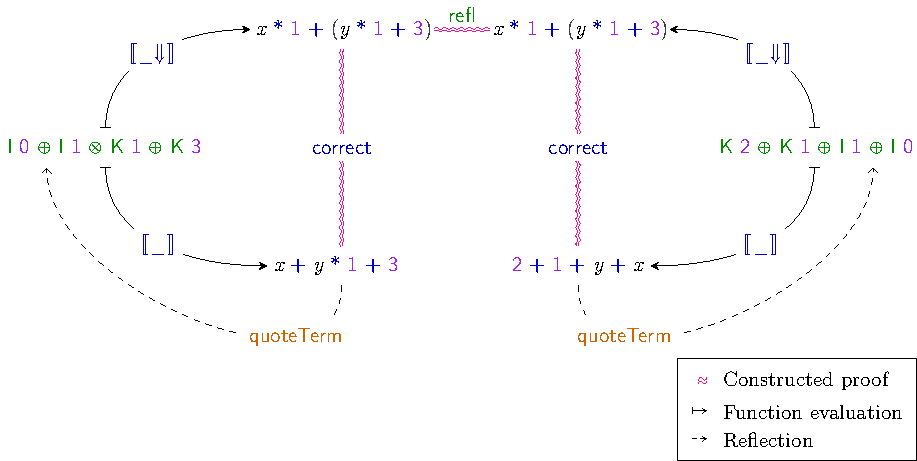
\includegraphics[draft=false]{graphics/reflexive-process}}
  \vspace*{-50pt}
  \caption{The Reflexive Proof Process}
  \label{proof-process}
\end{figure}

The identity we'll be working with is the lemma in Fig.~\ref{comparison}: the
left and right hand side of the equality are at the bottom of the diagram. Our
objective is to link those two expressions up through repeated application of
the ring axioms. We do this by converting both expressions to a normal form
(seen at the top of the diagram), and then providing a proof that this
conversion is correct according to the ring axioms (the
\(\AgdaFunction{correct}\) function in the diagram). Finally, we link up all of
these proofs, and if the two normal forms are definitionally equal, the entire
thing will typecheck, and we will have proven the equality.
\subsection{The \(\AgdaDatatype{Expr}\) AST}
In Agda, we can't manipulate the expressions we want to prove directly: instead,
we will construct an AST for each expression, and then do our manipulation on
that.

The AST type (\(\AgdaDatatype{Expr}\)) has a constructor for each of the ring
operators, as well as constructors for both variables and constants. The ASTs
for both expressions we want to prove can be seen on either side of
Fig.~\ref{proof-process}. Constants are constructed with
\(\AgdaInductiveConstructor{K}\), and variables are referred to by their de
Bruijn index (so \(x\) becomes \(\AgdaInductiveConstructor{I} \;
\AgdaNumber{0}\)).

From here, we can ``evaluate'' the AST in one of two ways: in a non-normalized
way (\(\AgdaFunction{⟦\_⟧}\)), or in a normalizing way
(\(\AgdaFunction{⟦\_⇓⟧}\)). This means that the goal of the
\(\AgdaFunction{correct}\) function is to show equivalence between
\(\AgdaFunction{⟦\_⟧}\) and \(\AgdaFunction{⟦\_⇓⟧}\).

Finally, we \emph{don't} want to force users to construct the
\(\AgdaDatatype{Expr}\) AST themselves. This is where reflection comes in: it
automates this construction (the path labeled \(\AgdaKeyword{quoteTerm}\) in the
diagram) from the goal type.
\subsection{Almost Rings}
While the stated domain of the solver is simply ``commutative rings'', it turns
out that we can be slightly more flexible than that if we pick our algebra
carefully.
As in \citet[section~5]{gregoire_proving_2005}, we use an algebra called an
\emph{almost-ring}. It has the regular operations (\(+\), \(*\)
(multiplication), \(-\), \(0\), and \(1\)), such that the following equations
hold:
\begin{align}
  0 + x       &= x \\
  x + y       &= y + x \\
  x + (y + z) &= (x + y) + z \\
  1 * x       &= x \\
  x * y       &= y * x \\
  x * (y * z) &= (x * y) * z \\
  (x + y) * z &= x * z + y * z \\
  0 * x       &= 0 \label{semiring} \\
  -(x * y)    &= - x * y \label{ringmul} \\
  -(x + y)    &= -x + -y \label{ringadd} \\
  \intertext{
  The equations up to \ref{semiring} represent a pretty standard definition of
  a (commutative) semiring. From there, though, things are different. The normal
  definition of a commutative ring would have (instead of \ref{ringmul} and
  \ref{ringadd}) the following:
  } 
  x + - x     &= 0
\end{align}
However, by choosing these slightly more complex laws, we can admit types like
\(\Nat\) which don't have additive inverses. Instead, these types can simply
supply the identity function for \(-\), and then \ref{ringmul} and \ref{ringadd}
will still hold.

A potential worry is that because we don't require \(x + -x = 0\) axiomatically,
it won't be provable in our system. Happily, this is not the case: as long as
\(1 + -1\) reduces to \(0\) in the coefficient set, the solver will verify the
identity.

In the library, the algebra is represented by the
\(\AgdaDatatype{AlmostCommutativeRing}\) type, a record with fields for each of
the ring axioms, defined over a user-supplied equivalence relation. Just as in
Agda's current solver, we also ask for one extra function: a weakly decidable
predicate to test if a constant is equal to zero.

\begin{centering}
  \ExecuteMetaData[../ReflexiveProcessRings.tex]{weak-dec}
\end{centering}

This function is used to speed up some internal algorithms in the solver, but it
isn't an essential component. By making it \emph{weakly} decidable, we allow
users to skip it
(\(\AgdaFunction{is-zero}~=~\AgdaFunction{const}~\AgdaInductiveConstructor{nothing}\))
if their type doesn't support decidable equality, or provide it (and get the
speedup) if it does.
\section{The Interface}
A decent interface is crucial if we want the solver to be broadly useful. We
strove to make our interface as simple and \emph{small} as possible. Aside from
the \(\AgdaDatatype{AlmostCommutativeRing}\) type described above, the
user-facing portion of our library consists of just two macros:
\(\AgdaMacro{solve}\) and \(\AgdaMacro{solveOver}\). Each of these infer the
goal from their context, and automatically construct the required machinery to
prove the equality.

\(\AgdaMacro{solve}\) is demonstrated in Fig.~\ref{the-solver}. It takes a
single argument: an implementation of the algebra. \(\AgdaMacro{solveOver}\) is
designed to be used in conjunction with manual proofs, so that a programmer can
automate a ``boring'' section of a larger more complex proof. It is called like
so:

\begin{centering}
  \ExecuteMetaData[../ReflectionSection.tex]{partial-auto}
\end{centering}

As well as the \(\AgdaDatatype{AlmostCommutativeRing}\) implementation, this
macro takes a list of free variables to use to compute the solution.

Because this interface is quite small, it's worth pointing out what's missing,
or rather, what we \emph{don't} require from the user:

\begin{itemize}
  \item We don't ask the user to construct the \(\AgdaDatatype{Expr}\) AST which
    represents their proof obligation. Compare this to Fig.~\ref{old-solver}: we
    had to write the type of the proof twice (once in the signature and again in
    the AST), and we had to learn the syntax for the solver's AST. 

    As well as being more verbose, this approach is less composable: every
    change to the proof type has to be accompanied by a corresponding change in
    the call to the solver. In contrast, the call to \(\AgdaMacro{solveOver}\)
    above effectively amounts to a demand for the compiler to ``figure it out!''
    Any change to the expressions on either side will result in an
    \emph{automatic} change to the proof constructed.
  \item We don't ask the user to write any kind of ``reflection logic'' for
    their type. In other words, we don't require a function which (for instance)
    recognizes and parses the user's type in the reflected AST, or a function
    which does the opposite, converting a concrete value into the AST that (when
    unquoted) would produce an expression equivalent to the quoted value.

    This kind of logic is complex, and very difficult to get right. While some
    libraries can assist with the task \citep{hinze_engineering_2013,
      norell_agda-prelude_2018} it is still not fully automatic.
\end{itemize}

Finally, despite the simplicity and ease-of-use described above, the solver is
\emph{not} specialized to a small number of types like \(\Nat\) and
so on. The whole library, including the reflection-based interface, will work
with any type with an \(\AgdaDatatype{AlmostCommutativeRing}\) instance.

\subsection{Reflection}
Agda has good support for reflection, which we will use to build our interface.
Agda's reflection system consists of three main parts: 
\begin{description}
  \item[\(\AgdaDatatype{Term}\)] The representation of Agda's AST, retrievable
    via \(\AgdaKeyword{quoteTerm}\).
  \item[\(\AgdaDatatype{Name}\)] The representation of identifiers, retrievable
    via \(\AgdaKeyword{quote}\).
  \item[\(\AgdaDatatype{TC}\)] The type-checker monad, which includes scoping
    and environment information, can raise type errors, unify variables, or
    provide fresh names. Computations in the \(\AgdaDatatype{TC}\) monad can be
    run with \(\AgdaKeyword{unquote}\).
\end{description}

While \(\AgdaKeyword{quote}\), \(\AgdaKeyword{quoteTerm}\), and
\(\AgdaKeyword{unquote}\) provide all the functionality we need, they're
somewhat low-level and noisy (syntactically speaking). Agda also provides a
mechanism (which it calls ``macros'') to package metaprogramming code so it
looks like a normal function call (as in \(\AgdaMacro{solve}\)).

Reflection is obviously a powerful tool, but it has a reputation for being
unsafe and error-prone. Agda's reflection system doesn't break type safety, but
we \emph{are} able to construct \(\AgdaDatatype{Term}\)s which are ill-typed,
which often result in confusing error-messages on the user's end. Unfortunately,
constructing ill-typed terms is quite easy to do: every quoted expression comes
with heaps of contextual information, making the whole thing very fragile.
Variables, for instance, are referred to by their de Bruijn indices, meaning
that the same \(\AgdaDatatype{Term}\) can break if it's simply moved under a
lambda.

All of that considered, we feel we managed to construct a reasonably robust
reflection-based interface. In doing so, we came up with the following general
guidelines for metaprogramming in Agda:

\begin{description}
  \item[Supply the minimal amount of information.] There were several instances
    where, in constructing a term, we were tempted to supply explicitly some
    argument that Agda usually infers. Universe levels were a common example.
    In general, though, this is a bad idea: AST manipulation is fragile and
    error-prone, so the chances that you'll get some argument wrong are very
    high. Instead, you should \emph{leverage} the compiler, relying on inference
    over direct metaprogramming as much as possible.
  \item[Don't assume structure.] A common pattern we used to try and find
    arguments to an \(n\)-ary function was to simply extract the last \(n\)
    visible arguments to the function. While in theory we might be able to
    statically know all of the implicit and explicit arguments that will be used
    at the call-site, it's much simpler to ignore them, and try our best to be
    flexible. Remember, none of this is typed, so if something changes (like,
    say, a new universe level in \(\AgdaDatatype{AlmostCommutativeRing}\)) in
    the order of arguments, you'll get type errors where you call
    \(\AgdaMacro{solve}\), not where it's implemented.
  \item[Ask for forgiveness, not permission.] We could also here say ``don't
    roll your own typechecker''. While it may seem good and fastidious to
    rigorously check the structure of the arguments given to a macro, often we
    found better results by assuming the argument was correct (where possible),
    and then carefully structuring the output in such a way to funnel a type
    error to the place where the input was incorrect. For instance, one section
    of the solver algorithm expects a proof that the two normal forms of the
    equations are the same. Here, we simply supply
    \(\AgdaInductiveConstructor{refl}\), assuming that they are, in fact, the
    same. When they're \emph{not}, for instance, in the following type:

    \begin{center}
      \ExecuteMetaData[../ReflectionSection.tex]{wrong-lemma}
    \end{center}

    A call to \(\AgdaMacro{solve}\) will provide the reasonably helpful error
    message:
    \[ x \neq y \; \text{of type} \; \AgdaDatatype{ℕ} \]
  \item[Try and implement as much of the logic outside of reflection
    as possible] Finally, after all of that, we advise minimizing the amount of
    actual metaprogramming code in a program, and confining it to the edges as
    much as possible. With great power comes poor error messages, fragility, and
    a loss of first-class status. Therefore, If something can be done without
    reflection, \emph{do it}, and use reflection as the glue to get from one
    standard representation to another.
\end{description}

At the core of the implementation you will find the following function:

\begin{center}
  \ExecuteMetaData[../ReflectionSection.tex]{to-expr}
\end{center}

This function is called on the \(\AgdaDatatype{Term}\) representing one side of
the target equality. It converts it to the corresponding
\(\AgdaDatatype{Expr}\). In other words, it performs the following
transformation:
\[
  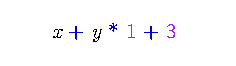
\includegraphics[trim={25 15 28 10}]{graphics/lhs-expr}
  \mapsto
  
\includegraphics[trim={25 15 22 10}]{graphics/lhs-ast}
\]


It also demonstrates the principles described above. The first four clauses all
match for the ring operators. Taking exponentiation as an example, it calls off
to the \(\AgdaFunction{getExp}\) function, which is implemented as follows:
\begin{center}
  \ExecuteMetaData[../ReflectionSection.tex]{getExp}
\end{center}
As described above, this function looks only for the last two visible arguments
to the exponentiation operator, ignoring all else. When it finds them, it
applies the corresponding constructor for \(\AgdaDatatype{Expr}\), using the
\(\AgdaFunction{⋯⟅∷⟆}\) function, which fills in all the hidden arguments we
want the compiler to infer.

Looking back to \(\AgdaFunction{toExpr}\), we notice that the last line is a
catch-all, which simply constructs a constant expression. This is the trick
which lets us avoid any custom quotation machinery from the user. It's also more
robust than asking for custom quotation machinery: if, for instance, there's a
function call or something similar hidden in this case, quotation won't work.
This solution, though, which just packages up the expression as-is, will have no
trouble.
\section{Performance}
Type-checking proof-heavy Agda code is notoriously slow, so the solver had to be
carefully optimized to avoid being so slow as to be unusable. We'll start by
first describing the unoptimized solver, and demonstrate how to improve its
performance iteratively.
\subsection{Horner Normal Form}
The representation used in Agda's current ring solver (and the one we'll start
out with here) is known as Horner Normal Form. A polynomial (more specifically,
a monomial) in \(x\) is represented as a list of coefficients of increasing
powers of \(x\). As an example, the following polynomial:
\begin{align}
  3 + 2x^2 + 4x^5 + 2x^7 \label{example-poly}
\end{align}
Is represented by the following list:
\[3, 0, 2, 0, 0, 4, 0, 2\]
Operations on these polynomials are similar to operations in positional number
systems.
\begin{center}
  \ExecuteMetaData[../HornerNormalForm.tex]{impl}
\end{center}
And finally, evaluation of the polynomial (given \(x\)) is a classic example of
the \(\AgdaFunction{foldr}\) function.
\begin{center}
  \ExecuteMetaData[../HornerNormalForm.tex]{eval}
\end{center}
\subsection{Sparse Encodings}
Our first avenue for optimization comes from \citet{gregoire_proving_2005}. Our
list encoding above is quite wasteful: it always stores an entry for each
coefficient, even if it's zero. Since expressions with long strings of zeroes
are common (things like \(x^{10}\)), it stands to reason that removing them
should improve performance.

The solution is to store what's known as a ``power index'' with every
coefficient. Intuitively, you can think of it as the ``distance to the next
non-zero coefficient''. Taking \ref{example-poly} again as an example, we would
now represent it as follows:
\[ (3,0),(2,1),(4,2),(2,1) \]

In Agda, we can go one step further, by disallowing zeroes in the representation
altogether. This statically ensures that the polynomial is always in its
smallest possible form. We don't include that detail here (it is in the
library), instead we will use this somewhat simplified type:
\begin{center}
  \ExecuteMetaData[../HornerNormalForm.tex]{sparse-poly}
\end{center}

Next, we turn our attention to the task of adding multiple variables. Luckily,
there's an easy way to do it: nesting. The idea is that a polynomial in \(n\)
variables is the same as before, except that its coefficients are themselves
polynomials in \(n-1\) variables. A polynomial in \(0\) variables in just a
constant. It's perhaps more clearly expressible in types:
\begin{center}
  \ExecuteMetaData[../HornerNormalForm.tex]{multi}
\end{center}

Before jumping into proving this, though, it's worth noting that another
opportunity for a ``sparse'' encoding has arisen. This time, polynomials which
don't include every variable contain gaps. In a polynomial of \(n\) variables,
a constant will always be stored behind \(n\) layers of nesting (we also prove
that this minimal form is maintained).

The solution is another index: this time an ``injection'' index. This represents
``how many variables to skip over before you get to the interesting stuff''.
This particular optimization is considerably more complex than the previous,
though: the number of variables in a polynomial is a type-relevant piece of
information, so any \emph{manipulation} of that index will have to justify
itself to the typechecker.
\subsection{Hanging Indices}
The problem is a common one: we have a piece of code that works efficiently,
and we now want to make it ``more typed'', by adding more information to it,
\emph{without} changing the complexity class or slowing it down.

We found the following strategy to be useful: first, write the untyped version
of the code, forgetting about the desired invariants as much as possible. Then,
to add the extra type information, look for an inductive type which participates
in the algorithm, and see if you can ``hang'' some new type indices off of it.

In our case, the injection index (distance to the next ``interesting''
polynomial) was simply stored as an \(\Nat\), and the information we
needed was the number of variables in the inner polynomial, and the number of
variables in the outer. All of that is stored in the following proof of \(\le\):

\begin{center}
  \ExecuteMetaData[../EfficiencyInIndexedTypes.tex]{leq-3}
\end{center}

A value of type \(n \; \AgdaDatatype{≤} \; m\) mimics the inductive structure of
the \(\Nat\) we were storing to represent the distance between \(n\)
and \(m\). We were able to take this analogy to the extreme: where we needed an
equivalent of \(\AgdaDatatype{Ordering}\):

\begin{center}
  \ExecuteMetaData[../EfficiencyInIndexedTypes.tex]{ord-type}
\end{center}

We were able to construct one, with transitivity replacing addition.

\begin{multicols}{2}
  \ExecuteMetaData[../EfficiencyInIndexedTypes.tex]{leq-compare}
\end{multicols}
\subsection{Unification}
So far, our optimizations have focused on the \emph{operations} performed on the
polynomial. Remember, though, the reflexive proof process has several steps:
only one of them containing the operations (\(\AgdaFunction{⟦\_⇓⟧}\) in
figure~\ref{proof-process}).

As it happens, we have now optimized these operations so much that they are no
longer the bottleneck in the process. Surprisingly, the innocuous-looking
\(\AgdaInductiveConstructor{refl}\) now takes the bulk of the time! Typechecking
this step involves unifying the two normalised expressions, a task which is
quite expensive, with counterintuitive performance characteristics. So
counterintuitive, in fact, that early versions of the solver, with all the
optimizations from \citet{gregoire_proving_2005} applied, was in many cases
\emph{slower} than the old, unoptimized solver!

In this section, we'll try and explain the problem and how we fixed it, and give
general guidelines on how to write Agda code which typechecks quickly.

First, the good news. In the general case, unifying two expressions takes time
proportional to the size of those expressions, so our hard-won optimizations do
indeed help us.

Unfortunately, though, the ``general case'' isn't really that general: Agda's
unification algorithm has a very important shortcut which we \emph{must} make
use of if we want our code to typecheck quickly: \emph{syntactic equality}.

Because Agda is a dependently-typed language, types can contain functions,
variables, and all sorts of complex expressions. One might expect that the
unification algorithm should compute these expressions as far as it can, getting
them to normal form, before it checks for any kind of equality. This would be
disastrous for performance! Consider the following:
\[ \AgdaFunction{sum} \; [ \AgdaNumber{1} .. \AgdaNumber{100} ] \stackrel{?}{=}
  \AgdaFunction{sum} \; [ \AgdaNumber{1} .. \AgdaNumber{100} ] \]

Running both computations here is an unnecessarily expensive task, and one which
Agda does indeed avoid. Before the full unification algorithm, the typechecker
does a quick pass to spot any syntactic equalities like the one above: if it
sees one, it can avoid any more computation on that particular expression.

Crucially, missing syntactic equality on a term doesn't just hurt performance
once: once syntactic equality fails, the next step is normalisation, which can
change the shape of the entire subexpression, \emph{destroying} any chance for
syntactic equality later on. This can result in a cascade of missed syntactic
equalities, causing a serious performance problem.

With that in mind, our optimisation will consist of two main strategies.
\subsubsection{Avoiding Progress}
First, we will consider something which may seem inconsequential: the order of
arguments to the evaluation functions.
\begin{multicols}{2}
  \centering
  \ExecuteMetaData[../PerformanceOfTypeChecking.tex]{forwards-eval}
  \ExecuteMetaData[../PerformanceOfTypeChecking.tex]{backwards-eval}
\end{multicols}
The definition on the left is the one we've been working with so far. To a
seasoned functional programmer, however, the version on the right might seem
much more natural. By one measure, the version on the right is better! When
applied to \(x^2 + 2\), it gives a much smaller normal form:
\begin{multicols}{2}
  \centering
  \ExecuteMetaData[../PerformanceOfTypeChecking.tex]{for-progress}
  \ExecuteMetaData[../PerformanceOfTypeChecking.tex]{back-progress}
\end{multicols}
Surprisingly, this is exactly what we \emph{don't} want! The left-hand-side
equation above, though larger, \emph{starts} with all of the variables, which
must be trivially equal to the same variables in the other expression. Since the
equality check proceeds left-to-right, this maintains that syntactic equality
for as long as possible.

On the right hand side, however, we first examine the coefficients. These are
computed from manipulations of the Horner Normal Form, and so are likely to be
\emph{not} syntactically equal. Even worse: since the expression \emph{can} be
normalised, we'll mess up its whole structure, ruining later syntactic checks!
\subsubsection{Avoiding Identities}

\subsection{Benchmarks}
\begin{figure}[h]
  \centering
  \newcounter{realxtickpos}
  \pgfplotsset{
      tick label style={font=\scriptsize},
      extra y tick style={yticklabel pos=right},
      title style={at={(-0.03,1.05)},anchor=west},
      xticklabel={%
        \ifnum \value{realxtickpos}=0%
          {$d = \pgfmathprintnumber{\tick}$}
        \else
          {$\pgfmathprintnumber{\tick}$}
        \fi
        \stepcounter{realxtickpos}
      },
      width=1.2\linewidth,
  }
  \setcounter{realxtickpos}{0}
  \begin{subfigure}[t]{0.3\linewidth}
    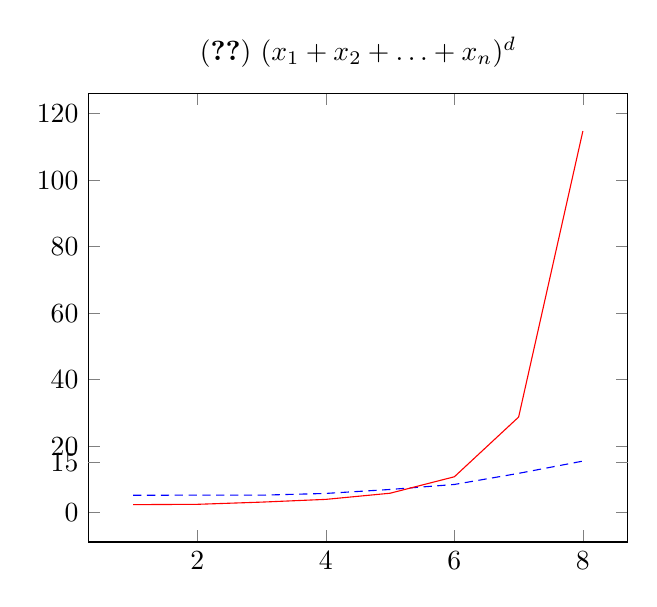
\begin{tikzpicture}
      \begin{axis}[
        legend columns=-1,
        legend entries={sparse, dense},
        legend to name=benchplots,
        extra y ticks={15},
        title={(\subref{bench1}) $(x_1 + x_2 + \ldots + x_n)^d$},
        ]
        \addplot[color=blue, densely dashed] coordinates{
          (1,5.20338)
          (2,5.25787)
          (3,5.24173)
          (4,5.76486)
          (5,6.95739)
          (6,8.46202)
          (7,11.8039)
          (8,15.4919)
        };
        \addplot[color=red] coordinates{
          (1,2.39014)
          (2,2.48972)
          (3,3.15072)
          (4,3.97797)
          (5,5.82725)
          (6,10.7788)
          (7,28.7441) 
          (8,114.779)
        };
      \end{axis}
    \end{tikzpicture}
    \phantomcaption \label{bench1}
  \end{subfigure}
  \setcounter{realxtickpos}{0}
  \begin{subfigure}[t]{0.3\linewidth}
    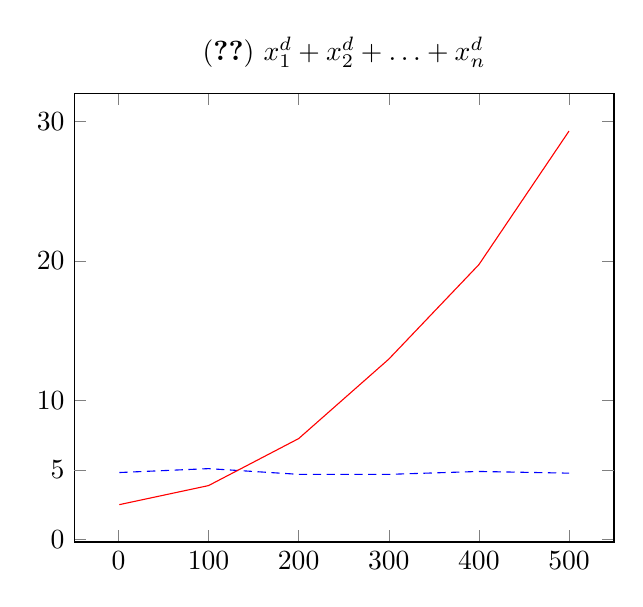
\begin{tikzpicture}
      \begin{axis}[
        extra y ticks={5},
        title={(\subref{bench2}) $x_1^d + x_2^d + \ldots + x_n^d$},
        ]
        \addplot[color=blue, densely dashed] coordinates{
          (  1,4.81414)
          (100,5.09434)
          (200,4.68453)
          (300,4.68257)
          (400,4.89147)
          (500,4.76918)
        };
        \addplot[color=red] coordinates{
          (  1, 2.50799)
          (100, 3.87669)
          (200, 7.25199)
          (300, 12.9566)
          (400, 19.7438)
          (500, 29.3335)
        };
      \end{axis}
    \end{tikzpicture}
    \phantomcaption\label{bench2}
  \end{subfigure}
  \setcounter{realxtickpos}{0}
  \begin{subfigure}[t]{0.3\linewidth}
    \begin{tikzpicture}
      \begin{axis}[
        extra y ticks={40},
        title={(\subref{bench3}) $(x_1^n + x_2^{n-1} + \ldots + x_n^1 + 1)^d$},
        ]
        \addplot[color=blue, densely dashed] coordinates{
          (1,5.999906778335571)
          (2,6.715672254562378)
          (3,6.018649101257324)
          (4,6.955428123474121)
          (5,9.579402923583984)
          (6,13.56689715385437)
          (7,23.99260210990906)
          (8,40.36761021614075)
        };
        \addplot[color=red] coordinates{
          (1,2.9551851749420166)
          (2,3.0478131771087646)
          (3,4.187927961349487)
          (4,6.412783861160278)
          (5,16.242217779159546)
          (6,49.26663112640381)
          (7,234.22495794296265)
          (8,1348.8776309490204)
        };
      \end{axis}
    \end{tikzpicture}
    \phantomcaption\label{bench3}
  \end{subfigure}

  \ref{benchplots}

  \caption{Time (in seconds) to prove each expression is equal to its expanded
    form ($n = 5$ for each).}
  \label{benchmarks}
\end{figure}
\section{Pedagogical Solutions}
One of the most widely-used and successful computer algebra systems, especially
among non-programmers, is Wolfram|Alpha
\cite{wolfram_research_inc._wolframalpha_2019}. It can generate ``pedagogical''
(step-by-step) solutions to maths
problems \cite{the_development_team_step-by-step_2009}. For instance, given the
input \(x^2 + 5 x + 6 = 0\), it will give the following output:
\begin{align*}
  x^2 + 5x + 6   = 0 \\
  (x + 2)(x + 3) = 0 \\
  x + 2 = 0   \; \text{or} \; x + 3 = 0 \\
  x     = -2  \; \text{or} \; x + 2 = 0 \\
  x     = -2  \; \text{or} \; x     = -3
\end{align*}

These tools can be invaluable for students learning basic mathematics.
Unfortunately, much of the software capable of generating usable solutions is
proprietary (including Wolfram Alpha), and little information is available as to
their implementation techniques.\cite{lioubartsev_constructing_2016} is perhaps
the best current work on the topic, but even so very little work exists in the
way of the theoretical basis for pedagogical solutions.

\citet{lioubartsev_constructing_2016} reformulates the problem as one of
\emph{pathfinding}. The left-hand-side and right-hand-side of the equation are
vertices in a graph, where the edges are single steps to rewrite an expression
to an equivalent form. A* is used to search.

This approach suffers from a huge search space: every vertex will have an edge
for almost every one of the ring axioms, and as such a good heuristic is
essential. Unfortunately, what this should be is not
clear: \citet{lioubartsev_constructing_2016} uses a measure of the ``simplicity''
of an expression.

So, with an eye to using our solver instead of A*, we can notice that paths in
undirected graphs form a perfectly reasonable equivalence relation: transitivity
is the concatenation of paths, reflexivity is the empty path, and symmetry is
\emph{reversing} a path. Equivalence classes, in this analogy, are connected
components of the graph.

More practically speaking, we implement these ``paths'' as lists, where the
elements of the list are elementary ring axioms. When we want to display a
step-by-step solution, we simply print out each element of the list in turn,
interspersed with the states of the expression (the vertices in the graph).
\begin{multicols}{2}
  \ExecuteMetaData[../SetoidApplications.tex]{traced}
\end{multicols}

If we stopped there, however, the solver would output incredibly verbose
``solutions'': far too verbose to be human-readable. Instead, we must apply a
number of heuristics to cut down on the solution length:
\begin{wrapfigure}{r}{0.5\linewidth}
  \centering
  \begin{tikzpicture}
    \node (n0) at (2,9) {$1 + 2 + y + x$};
    \node (n1) at (-2,6) {$x + y * 1 + 3$};
    \node (n2) at (2,7.5) {$3 + y + x$};
    \node (n3) at (2,6) {$y + 3 + x$};
    \node (n4) at (0,4.5) {$x + y + 3$};
    \node (n5) at (-1,3) {$3 + x + y$};
    \node (n6) at (1,3) {$x + 3 + y$};
    \draw[-stealth] (n1) to (n4);
    \draw[-stealth] (n3) to (n2);
    \draw[-stealth] (n2) to (n0);
    \draw[-stealth] (n4) to (n3);
    \draw[-stealth] (n4) to (n5);
    \draw[-stealth] (n5) to (n6);
    \draw[-stealth] (n6) to (n4);
  \end{tikzpicture}
  \caption{Hourglass-Shaped Graph}
  \label{h-graph}
\end{wrapfigure}
\begin{enumerate}
  \item First, we filter out ``uninteresting'' steps. These are steps which are
    obvious to a human, like associativity, or evaluation of closed terms. When
    a step is divided over two sides of an operator, it is deemed
    ``interesting'' if either side is interesting.
  \item Next, we remove any ``step, reverse-step'' chains. Since we're
    converting expressions to normal form, the path may be hourglass-shaped.
    Fig.~\ref{h-graph} is the output from our solver without this heuristic
    applied.

    The problem is that both expressions hit a common form early on, at \(x + y
    + 3\). Nonetheless, the proof will soldier on, giving superfluous steps.

    These sections are what we want to detect, and remove.
\end{enumerate}

After applying those heuristics, our solver outputs the following for the lemma
in Fig.~\ref{the-solver}:
\begin{center}
\begin{BVerbatim}
x + y * 1 + 3
    ={ eval }
x + y + 3
    ={ +-comm(x,y + 3) }
y + 3 + x
    ={ +-comm(y,3) }
3 + y + x
    ={ eval }
2 + 1 + y + x
\end{BVerbatim}
\end{center}
Figuring out good heuristics and path compression techniques seems to deserve
further examination.
\section{Related Work}
In dependently-typed programming languages, the state-of-the-art solver for
polynomial equalities (over commutative rings) was originally presented
in \citet{gregoire_proving_2005}, and is used in Coq's \verb+ring+ solver. This
work improved on the already existing solver \cite{Coq:manual} in both efficiency
and flexibility. In both the old and improved solvers, a reflexive technique is
used to automate the construction of the proof obligation (as described in
\citet{boutin_using_1997}).

Agda \cite{norell_dependently_2008} is a dependently-typed programming language
based on Martin-Löf's Intuitionistic Type
Theory \cite{martin-lof_intuitionistic_1980}. Its standard
library \cite{danielsson_agda_2018} currently contains a ring solver which is
similar in flexibility to Coq's \verb+ring+, but doesn't support the
reflection-based interface, and is less efficient to the one presented here. 

In \citet{geuvers_automatically_2017}, an implementation of an automated solver
for the dependently-typed language Idris \cite{brady_idris_2013} is described.
The solver is implemented with a ``correct-by-construction'' approach, in
contrast to \citet{gregoire_proving_2005}. The solver is defined over
\emph{non}commutative rings, meaning that it is more general (can work with more
types) but less powerful (meaning it can prove fewer identities). It provides a
reflection-based interface, but internally uses a dense representation.

Reflection and metaprogramming are relatively recent additions to Agda, but form
an important part of the interfaces to automated proof procedures. Reflection in
dependent types in general is explored in \citet{christiansen_practical_2015},
and specific to Agda in \citet{van_der_walt_reflection_2012}.

Formalization of mathematics in general is an ongoing project.
\citet{wiedijk_formalizing_2018} tracks how much of ``The 100 Greatest Theorems''
\cite{kahl_hundred_2004} have so far been formalized (at time of writing, the
number stands at 93). DoCon \cite{meshveliani_docon-provable_2018} is a notable
Agda library in this regard: it contains many tools for basic maths, and
implementations of several CAS algorithms. Its implementation is described
in \citet{meshveliani_dependent_2013}. \citet{cheng_functional_2018} describes the
manipulation of polynomials in both Haskell and Agda.

Finally, the study of \emph{pedagogical} CASs which provide step-by-step
solutions is explored in \citet{lioubartsev_constructing_2016}. One of the most
well-known such system is Wolfram Alpha
\cite{wolfram_research_inc._wolframalpha_2019}, which has step-by-step solutions
\cite{the_development_team_step-by-step_2009}.

%% Acknowledgments
\begin{acks}                            %% acks environment is optional
                                        %% contents suppressed with 'anonymous'
  %% Commands \grantsponsor{<sponsorID>}{<name>}{<url>} and
  %% \grantnum[<url>]{<sponsorID>}{<number>} should be used to
  %% acknowledge financial support and will be used by metadata
  %% extraction tools.
  This material is based upon work supported by the
  \grantsponsor{GS100000001}{National Science
    Foundation}{http://dx.doi.org/10.13039/100000001} under Grant
  No.~\grantnum{GS100000001}{nnnnnnn} and Grant
  No.~\grantnum{GS100000001}{mmmmmmm}.  Any opinions, findings, and
  conclusions or recommendations expressed in this material are those
  of the author and do not necessarily reflect the views of the
  National Science Foundation.
\end{acks}


%% Bibliography
\bibliography{../bibliography.bib}
%% Appendix
\appendix
\section{Appendix}

Text of appendix \ldots

\end{document}
